\subsection{Delay-Doppler Domain Representation}

The analysis of high-mobility wireless channels requires a signal representation that can describe both multipath propagation and Doppler effects. Conventional multicarrier systems such as OFDM usually describe signal transmission in the time-frequency domain. This representation is convenient for practical implementation, because data symbols can be arranged over time slots and frequency subcarriers.

However, in high-mobility environments, the wireless channel may vary rapidly over time due to Doppler effects. As a result, the time-frequency channel coefficients can change significantly from one resource element to another. This makes channel estimation and equalization more difficult. For this reason, the delay-Doppler domain is introduced as an alternative representation that is more closely related to the physical propagation paths of the wireless channel.

The delay-Doppler representation is an important foundation for OTFS modulation. Instead of describing the channel only by its variations over time and frequency, this representation describes the channel using propagation delay and Doppler shift. These two quantities correspond directly to multipath propagation and relative motion, respectively.

\subsubsection{Time-Frequency Domain}

The time-frequency domain is widely used in modern wireless communication systems, especially in OFDM-based transmission. In this representation, the available transmission resources are divided into time slots and frequency subcarriers. Each information symbol is placed on a specific time-frequency resource element.

The time axis represents consecutive OFDM symbols or time slots, while the frequency axis represents the orthogonal subcarriers. Therefore, each cell in the time-frequency grid corresponds to one symbol position in both time and frequency. This structure is suitable for OFDM because one OFDM symbol occupies a time interval and contains multiple subcarriers in the frequency domain.

\begin{figure}[H]
\centering
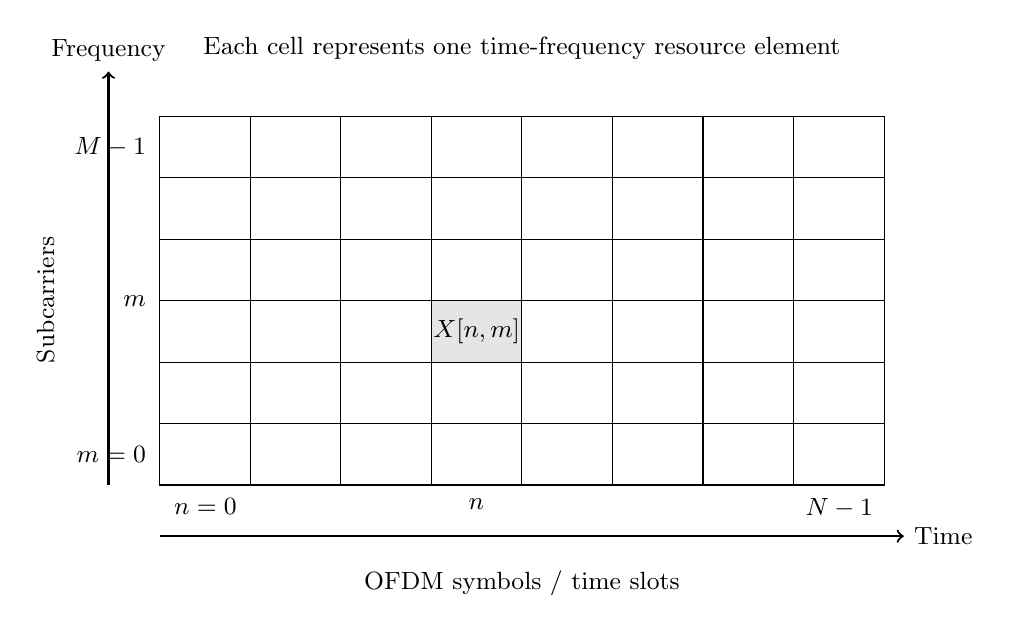
\begin{tikzpicture}[every node/.style={font=\small}]

    % Grid parameters
    \def\cw{1.15}
    \def\ch{0.78}

    % Draw grid
    \foreach \i in {0,...,7} {
        \foreach \j in {0,...,5} {
            \draw (\i*\cw,\j*\ch) rectangle ++(\cw,\ch);
        }
    }

    % Highlight one resource element
    \filldraw[fill=gray!20, draw=black] (3*\cw,2*\ch) rectangle ++(\cw,\ch);
    \node at (3*\cw+0.5*\cw,2*\ch+0.5*\ch) {$X[n,m]$};

    % Axes
    \draw[->, thick] (-0.65,0) -- (-0.65,5.25) node[above] {Frequency};
    \draw[->, thick] (0,-0.65) -- (9.45,-0.65) node[right] {Time};

    % Axis descriptors
    \node[rotate=90] at (-1.45,2.35) {Subcarriers};
    \node at (4.6,-1.25) {OFDM symbols / time slots};

    % Labels on vertical axis
    \node[left] at (-0.05,0.39) {$m=0$};
    \node[left] at (-0.05,2.34) {$m$};
    \node[left] at (-0.05,4.29) {$M-1$};

    % Labels on horizontal axis
    \node[below] at (0.58,-0.05) {$n=0$};
    \node[below] at (4.02,-0.05) {$n$};
    \node[below] at (8.63,-0.05) {$N-1$};

    % Top explanation
    \node at (4.6,5.55) {Each cell represents one time-frequency resource element};

\end{tikzpicture}
\caption{Time-frequency grid representation used in multicarrier transmission systems.}
\label{fig:time_frequency_grid}

\end{figure}

Figure~\ref{fig:time_frequency_grid} illustrates the time-frequency grid structure. In OFDM, data symbols are directly assigned to this grid. The receiver then processes the received signal in the frequency domain using FFT-based operations. This approach is effective when the channel is approximately constant during one OFDM symbol interval.

Nevertheless, the time-frequency representation becomes less stable in high-mobility environments. When the transmitter, receiver, or surrounding scatterers move rapidly, the channel changes during transmission. Consequently, the channel response in the time-frequency domain may fluctuate quickly across both time and frequency. This effect can destroy the orthogonality among OFDM subcarriers and introduce inter-carrier interference.

Although the time-frequency domain is convenient for waveform generation and practical implementation, it does not always provide the most compact description of doubly selective channels. This motivates the use of the delay-Doppler domain.

\subsubsection{Delay-Doppler Representation}

The delay-Doppler domain describes the wireless channel using two physical parameters: propagation delay and Doppler shift. The delay dimension is associated with multipath propagation. Different reflected paths travel different distances before reaching the receiver, so they arrive at different times. The Doppler dimension is associated with relative motion. When the transmitter, receiver, or scatterers are moving, each path may experience a frequency shift.

In this representation, each dominant propagation path can be described by three main parameters: its path gain, its delay, and its Doppler shift. Therefore, instead of viewing the channel as a rapidly changing surface over time and frequency, the delay-Doppler domain views it as a collection of physical propagation paths.

A simple delay-Doppler channel model can be expressed as

\begin{equation}
h(\tau,\nu)
=
\sum_{i=1}^{P}
h_i
\delta(\tau-\tau_i)
\delta(\nu-\nu_i),
\end{equation}

where \(P\) denotes the number of dominant propagation paths. The parameter \(h_i\) represents the complex gain of the \(i\)-th path, while \(\tau_i\) and \(\nu_i\) denote its delay and Doppler shift, respectively.

This equation means that the channel can be interpreted as the sum of several dominant propagation components. Each component appears at a certain delay and a certain Doppler shift. In many practical wireless channels, only a limited number of propagation paths carry significant energy. Therefore, the delay-Doppler channel representation is often sparse.

\begin{figure}[H]
\centering
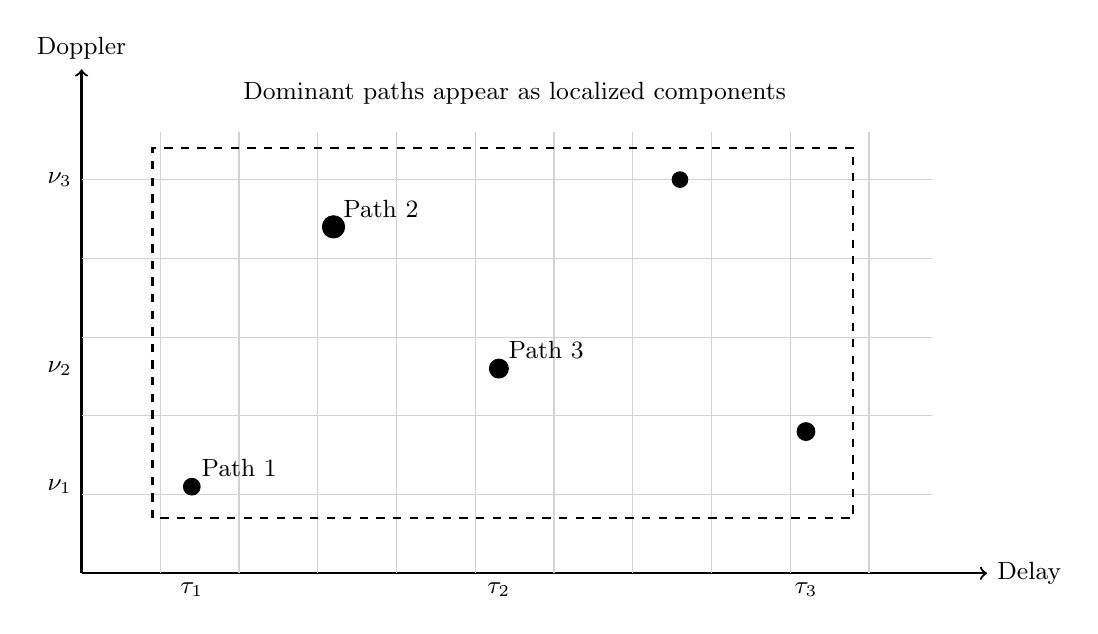
\begin{tikzpicture}[
every node/.style={font=\small},
axis/.style={->, thick},
gridline/.style={gray!35, thin}
]

    % Axes
    \draw[axis] (0,0) -- (11.5,0) node[right] {Delay};
    \draw[axis] (0,0) -- (0,6.4) node[above] {Doppler};

    % Grid
    \foreach \x in {1,2,...,10} {
        \draw[gridline] (\x,0) -- (\x,5.6);
    }

    \foreach \y in {1,2,3,4,5} {
        \draw[gridline] (0,\y) -- (10.8,\y);
    }

    % Sparse dominant paths
    \filldraw[black] (1.4,1.1) circle (3.0pt);
    \filldraw[black] (3.2,4.4) circle (4.0pt);
    \filldraw[black] (5.3,2.6) circle (3.4pt);
    \filldraw[black] (7.6,5.0) circle (2.8pt);
    \filldraw[black] (9.2,1.8) circle (3.2pt);

    % Path labels
    \node[above right] at (1.4,1.1) {Path 1};
    \node[above right] at (3.2,4.4) {Path 2};
    \node[above right] at (5.3,2.6) {Path 3};

    % Sparse support region
    \draw[dashed, thick] (0.9,0.7) rectangle (9.8,5.4);

    % Axis tick labels
    \node[below] at (1.4,0) {$\tau_1$};
    \node[below] at (5.3,0) {$\tau_2$};
    \node[below] at (9.2,0) {$\tau_3$};

    \node[left] at (0,1.1) {$\nu_1$};
    \node[left] at (0,2.6) {$\nu_2$};
    \node[left] at (0,5.0) {$\nu_3$};

    % Annotation
    \node[align=center] at (5.5,6.1)
    {Dominant paths appear as localized components};

\end{tikzpicture}
\caption{Sparse representation of dominant multipath components in the delay-Doppler domain.}
\label{fig:delay_doppler_channel}

\end{figure}

As illustrated in Fig.~\ref{fig:delay_doppler_channel}, each significant propagation path appears as a localized component in the delay-Doppler plane. The horizontal coordinate represents the propagation delay, while the vertical coordinate represents the Doppler shift. Since the number of dominant paths is usually limited, the channel energy is concentrated around several points or small regions.

This sparse representation is useful in high-mobility communications. In the time-frequency domain, the channel coefficients may vary rapidly due to Doppler effects. In the delay-Doppler domain, however, the physical path parameters usually vary more slowly. This makes the delay-Doppler domain more suitable for describing doubly selective wireless channels.

Compared with the time-frequency domain, the delay-Doppler domain provides a more compact and physically meaningful description of the wireless channel. This is one of the main motivations for OTFS modulation.

\subsubsection{Relationship Between Signal Domains}

The time-frequency and delay-Doppler domains are not independent representations. They describe the same wireless communication system from different viewpoints. The time-frequency domain is convenient for practical waveform generation, while the delay-Doppler domain is more suitable for describing physical channel behavior in high-mobility scenarios.

In conventional OFDM systems, information symbols are placed directly on the time-frequency grid. Each symbol is associated with a particular OFDM symbol index and subcarrier index. In contrast, OTFS places information symbols on the delay-Doppler grid first. These symbols are then transformed into the time-frequency grid before transmission.

This transformation is performed by the inverse symplectic finite Fourier transform (ISFFT). At the receiver, after the signal has passed through the wireless channel and has been processed in the time-frequency domain, the symplectic finite Fourier transform (SFFT) is used to transform the received samples back into the delay-Doppler domain.

Instead of presenting the full mathematical expressions of these transforms here, the main idea can be understood as follows. The ISFFT spreads each delay-Doppler symbol over the time-frequency plane before transmission. After reception, the SFFT collects the received time-frequency information back into the delay-Doppler domain. Therefore, the two transforms form a bridge between the physical delay-Doppler representation and the practical time-frequency transmission structure.

\begin{figure}[H]
\centering
\resizebox{0.96\linewidth}{!}{%
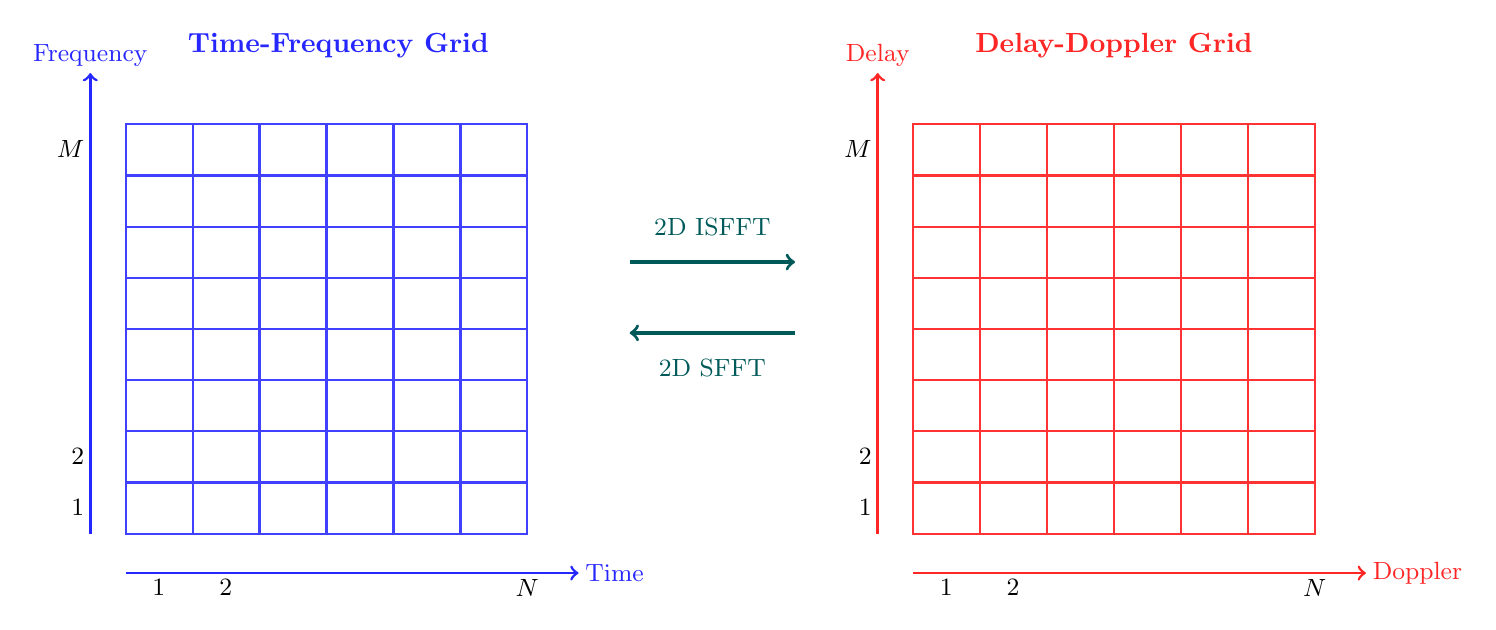
\begin{tikzpicture}[every node/.style={font=\small, inner sep=2pt}]

    % Parameters
    \def\cw{0.85}
    \def\ch{0.65}

    % =====================================================
    % Left grid: Time-Frequency
    % =====================================================
    \begin{scope}[shift={(0,0)}]

        \foreach \i in {0,...,5} {
            \foreach \j in {0,...,7} {
                \draw[blue!75, line width=0.8pt] (\i*\cw,\j*\ch) rectangle ++(\cw,\ch);
            }
        }

        \draw[->, blue!85, line width=1pt] (-0.45,0) -- (-0.45,5.85) node[above] {Frequency};
        \draw[->, blue!85, line width=1pt] (0,-0.5) -- (5.75,-0.5) node[right] {Time};

        \node[below] at (0.42,-0.5) {$1$};
        \node[below] at (1.27,-0.5) {$2$};
        \node[below] at (5.10,-0.5) {$N$};

        \node[left] at (-0.45,0.33) {$1$};
        \node[left] at (-0.45,0.98) {$2$};
        \node[left] at (-0.45,4.88) {$M$};

        \node[blue!85, font=\bfseries] at (2.7,6.2) {Time-Frequency Grid};

    \end{scope}

    % =====================================================
    % Middle arrows
    % =====================================================
    \draw[->, teal!70!black, line width=1.2pt] (6.4,3.45) -- (8.5,3.45);
    \node[teal!70!black] at (7.45,3.9) {2D ISFFT};

    \draw[->, teal!70!black, line width=1.2pt] (8.5,2.55) -- (6.4,2.55);
    \node[teal!70!black] at (7.45,2.1) {2D SFFT};

    % =====================================================
    % Right grid: Delay-Doppler
    % =====================================================
    \begin{scope}[shift={(10.0,0)}]

        \foreach \i in {0,...,5} {
            \foreach \j in {0,...,7} {
                \draw[red!80, line width=0.8pt] (\i*\cw,\j*\ch) rectangle ++(\cw,\ch);
            }
        }

        \draw[->, red!85, line width=1pt] (-0.45,0) -- (-0.45,5.85) node[above] {Delay};
        \draw[->, red!85, line width=1pt] (0,-0.5) -- (5.75,-0.5) node[right] {Doppler};

        \node[below] at (0.42,-0.5) {$1$};
        \node[below] at (1.27,-0.5) {$2$};
        \node[below] at (5.10,-0.5) {$N$};

        \node[left] at (-0.45,0.33) {$1$};
        \node[left] at (-0.45,0.98) {$2$};
        \node[left] at (-0.45,4.88) {$M$};

        \node[red!85, font=\bfseries] at (2.55,6.2) {Delay-Doppler Grid};

    \end{scope}

\end{tikzpicture}
}
\caption{Relationship between time-frequency and delay-Doppler signal domains.}
\label{fig:tf_dd_relationship}

\end{figure}

As illustrated in Fig.~\ref{fig:tf_dd_relationship}, the delay-Doppler grid and the time-frequency grid are connected through two-dimensional transforms. The delay-Doppler grid is useful for symbol placement and channel interpretation, while the time-frequency grid is suitable for practical transmission using multicarrier waveforms.

This relationship is particularly important for OTFS. OTFS does not completely discard the time-frequency domain. Instead, it uses the delay-Doppler domain for data representation and then maps the symbols into the time-frequency domain for transmission. In this way, OTFS can remain compatible with multicarrier transmission principles while exploiting the physical delay and Doppler characteristics of high-mobility wireless channels.

Table~\ref{tab:signal_domain_relationship} summarizes the main differences between the two domains.

\begin{table}[H]
\centering
\caption{Comparison between time-frequency and delay-Doppler signal domains.}
\label{tab:signal_domain_relationship}

\renewcommand{\arraystretch}{1.35}
\begin{tabularx}{\textwidth}{|
>{\RaggedRight\arraybackslash}p{3.0cm}|
>{\RaggedRight\arraybackslash}X|
>{\RaggedRight\arraybackslash}X|}
\hline
\textbf{Aspect} &
\textbf{Time-Frequency Domain} &
\textbf{Delay-Doppler Domain} \\
\hline

Signal coordinates &
Time and frequency indices &
Delay and Doppler indices \\
\hline

Typical use &
OFDM-based transmission &
OTFS-based transmission \\
\hline

Channel description &
Channel variation over time and frequency &
Physical paths with delay and Doppler shift \\
\hline

High-mobility behavior &
Rapidly varying channel coefficients &
Sparse and more stable path representation \\
\hline

Main transform &
FFT/IFFT operations &
SFFT/ISFFT operations \\
\hline

\end{tabularx}
\end{table}

Therefore, the delay-Doppler domain does not replace the time-frequency domain in practical implementation. Instead, it complements it. The time-frequency domain remains convenient for waveform generation and compatibility with OFDM architectures, while the delay-Doppler domain provides a more suitable representation for data placement and channel interpretation under high-mobility conditions. This idea forms the foundation of OTFS modulation, which is discussed in detail in Chapter 3.
